\let\cleardoublepage\clearpage
\chapter{Горное и нефтегазовое дело}

{\bfseries МРНТИ 52.13.23}
\hfill {\bfseries \href{https://doi.org/10.58805/kazutb.v.2.23-213}{https://doi.org/10.58805/kazutb.v.2.23-213}}

\sectionwithauthors{Р.А. Мусин, Ж.М. Асанова, М.А. Байкенжин, Р.Х. Альжанов}{ТЕХНОЛОГИЯ КРЕПЛЕНИЯ ВЕНТИЛЯЦИОННОГО СТВОЛА №3 МЕСТОРОЖДЕНИЯ
«ЖОМАРТ 2»}

\begin{center}
{\bfseries Р.А. Мусин, Ж.М. Асанова\textsuperscript{🖂}, М.А. Байкенжин, Р.Х. Альжанов}

Карагандинский технический университет имени Абылкаса Сагинова,

Караганда, Казахстан,

{\bfseries \textsuperscript{🖂}} Корреспондент-автор: e-mail: zhanar-a@bk.ru
\end{center}

Данная статья посвящена решению проблемы, имеющей важное практическое
значение такой, как повышение экономической и техникой эффективности
строительства и эксплуатации горных выработок, на которое направлено
теоретическое обобщение и научное обоснование инновационных проектных,
конструктивных и технологических решений в сфере крепления глубоких
вертикальных стволов.

Обычно технология проходки восстающих включает в себя бурение
направляющей скважины с верхнего горизонта вниз к существующей
выработке, затем снимается долото и устанавливается расширительная
головка. Нынешние уровни технологии позволяют легко провести восстающую,
3 -- 4 метра. Бурения восстающих выработок большего диаметра довольно
медленно осваивается, хотя усовершенствованные технологии буровых работ
и параметры расширительных головок дают возможность бурить выработки
диаметром 5 -- 6 метров с увеличенной производительностью и
положительным экономическим эффектом, чем в прошлом.

Технический результат заключается в повышении эффективности крепления
шахтного ствола за счет конструкции, включающей в себя кольцевую крепь,
размещённую в специальной нише ствола, закрепленную анкерами. Для
предотвращения вывалов породы, устанавливается сетка, в местах
геологических нарушений дополнительно применяется набрызгбетонная крепь.

{\bfseries Ключевые слова:} вентиляционный ствол, восстающие выработки,
расширяющие головки, бетонирование, армировка, набрызгбетон, кольцевая
крепь.

\begin{center}
{\large\bfseries «ЖОМАРТ 2» КЕН ОРНЫНЫҢ №3 ЖЕЛДЕТУ ОҚПАНЫН БЕКІТУ ТЕХНОЛОГИЯСЫ}

{\bfseries Р.А. Мусин, Ж.М.Асанова\textsuperscript{🖂}, М.А. Байкенжин, Р.Х.
Альжанов}

Әбілқас Сағынов атындағы Қарағанды техникалық университеті,

Қарағанды қ., Қазақстан,

e-mail: zhanar-a@bk.ru
\end{center}

Бұл мақала терең тік оқпандарды бекіту саласындағы Инновациялық жобалау
әдістерін, конструктивті және технологиялық шешімдерді теориялық
жалпылау мен ғылыми негіздеуге бағытталған қазбаларды салу мен
пайдаланудың техникалық-экономикалық тиімділігін арттыру сияқты маңызды
практикалық маңызы бар мәселені шешуге арналған.

Әдетте, көтерілісшілерді бұрғылау технологиясы бағыттаушы ұңғыманы
жоғарғы горизонттан қолданыстағы қазбаға дейін бұрғылауды қамтиды, содан
кейін қашау алынып, кеңейту басы орнатылады. Технологияның қазіргі
деңгейлері 3-4 метрге көтерілуді жеңілдетеді. Үлкен диаметрлі өрлемелі
қазбаларды бұрғылау өте баяу игерілуде, дегенмен кеңейту бастарының
конструкциялары мен жетілдірілген бұрғылау технологиялары 5-6 метрлік
бұрғылауға мүмкіндік береді, бұл бұрынғыға қарағанда өнімділігі мен
экономикалық тиімділігі жоғары.

Техникалық нәтиже якорьмен бекітілген арнайы оқпан тауашасына
орналастырылған сақиналы бекіткішті қамтитын конструкция есебінен шахта
оқпанын бекіту тиімділігін арттыру болып табылады. Тау жыныстарының
үйілуін болдырмау үшін тор орнатылады, геологиялық бұзылу орындарында
қосымша бетон бекіткіші қолданылады.

{\bfseries Түйін сөздер:} желдету стволы, жоғары қараған қазбалар, кеңейту
бастары, бетондау, арматура, бүріккішбетон, сақиналы бекіткіш.

\begin{center}
{\large\bfseries THE TECHNOLOGY OF FASTENING THE VENTILATION SHAFT No. 3 OF THE «JOMART 2» DEPOSIT}

{\bfseries R.A. Musin, Zh.M.Asanova\textsuperscript{🖂}, M.A. Baykenzhin,
R.H. Alzhanov}

Karaganda Technical University named after Abylkas Saginov,

Karaganda, Kazakhstan,

е-mail: zhanar-a@bk.ru
\end{center}

This article is devoted to solving a problem of great practical
importance, such as improving the technical and economic efficiency of
construction and operation of workings, which is aimed at theoretical
generalization and scientific justification of innovative design
methods, constructive and technological solutions in the field of
fastening deep vertical shafts.

Usually, the technology of sinking the rebels involves drilling a guide
well from the upper horizon down to the existing development, then the
chisel is removed and the expansion head is installed. Current levels of
technology make it easy to hold a rising, 3 -- 4 meters. Drilling of
rising workings of a larger diameter is being mastered rather slowly,
although the design of expansion heads and advanced drilling
technologies allow drilling with a diameter of 5-6 meters with greater
productivity and positive economic effect than in the past.

The technical result is to increase the efficiency of fixing the shaft
shaft due to the design, which includes an annular support placed in a
special niche of the shaft, secured with anchors. To prevent rock falls,
a grid is installed, in places of geological violations, a
spray-concrete support is additionally applied.

{\bfseries Keywords:} ventilation shaft, rising workings, expanding heads,
concreting, reinforcement, spray concrete, ring support.

\begin{multicols}{2}
{\bfseries Введение.} Цель. Кроме объективных горно-геологических посылов,
одной из оснований невысокой технико-экономической производительности
проходки, крепления и эксплуатации основательных стволов считается
внедрение закоренелых раскладов при их проектировании и строительстве.
Данные расклады базируются на неполных исходных данных и устаревших
нормативных основах, характеризуются широким применением схем проходки,
в сочетании с последующим усилением, ограниченным набором заключений по
увеличению несущей возможности укрепления, основанных на экстенсивных
принципах, недостающим учетом влияющих горнотехнических и
технологических моментов {[}1{]}.

Последние фундаментальные исследования в области геомеханики и
геотехнологии дают возможность признать, собственно что
высококачественное совершенствование производительности строительства и
эксплуатации основательных стволов вполне вероятно при переходе к
инновационным способам проектирования и строительства, учитывающего
выполнение системного анализа взаимодействия отдельных составляющих
геотехнических систем и интенсивное внедрение современных конструктивных
и технологических заключений на базе передовых средств укрепления
массива, высокоэффективных материалов укрепления, современных схем
проходки и др {[}2{]}.

Месторождение Жаман-Айбат находится в Улытауской области, Жанааркинском
районе, в 130 км от города Жезказган.

Месторождение пространственно приурочено горам Жаман-Айбат, которые
вытянуты а субширотном направлении и занимают площадь по середине
месторождения.

Стволы блока 19, 37 «Вентиляционный ствол №3, Жомарт 2 были пройдены
буровой установкой «RHINO 2007 DC». Для разработки технологического
регламента были предоставлены материалы по воздухоподающему стволу № 1
панели 37. Рассматриваемый

5-6 метров с положительным экономическим эффектом, чем это было ранее
{[}3{]}.

Ствол пройден в районе панели 37 в восточной части месторождения. Ствол
предназначен для подачи воздуха в шахту. Глубина ствола 490,72 м. Нижняя
отметка ствола 142,72 м. Диаметр ствола 4,5 м. Ствол был пройден в 2017
году. В настоящее время стенки ствола не закреплены.

Вентиляционные стволы являются неотъемлемой частью системы вентиляции
угольных шахт и рудников, работающих на больших глубинах. На текущий
момент подача воздуха в эти стволы осуществляется вентиляторными
установками с электродвигателями мощностью от 500 до 3000 кВт и более.
Однако их коэффициент полезного действия практически не превышает 0,35,
что означает, что около 65\% электроэнергии, потребляемой на вентиляцию,
теряется. Одной из причин этого является высокое аэродинамическое
сопротивление вентиляционных стволов, которые загромождены армировкой,
подъемными сосудами и коммуникациями {[}4{]}.

Для улучшения технико-экономической эффективности строительства и
эксплуатации вентиляционных стволов, прокладываемых в устойчивых
породах, рекомендуется использовать ресурсосберегающую набрызгбетонную
крепь или комбинированную крепь с гибкой армировкой в соответствии с
требованиями. Однако при глубинах стволов более 500 м применение гибкой
армировки становится затруднительным из-за большого веса канатов,
натяжных устройств, а также необходимости увеличения диаметра ствола,
если размеры поперечного сечения принимаются с учетом размеров подъемных
сосудов и соответствующих зазоров. В связи с этим на практике в глубоких
стволах широко используется монолитная бетонная крепь и жесткая
армировка, которые не соответствуют критериям технико-экономической
эффективности.

С увеличением глубины современных вертикальных стволов, усложнением
конструкции их армировки и ростом металлоемкости последней, данная
проблема становится все более актуальной {[}5{]}.

{\bfseries Материалы и методы.} Проходка восстающих выработок разного
предназначения всякий раз была делом дорогим, медленным и довольно
небезопасным. Наиболее часто применяемой технологией проходки восстающих
является метод, при котором изначально пробуривается направляющая
скважина с верхнего горизонта в направлении вниз к ранее пройденной
выработке (рисунок 1).
\end{multicols}

\begin{figure}[H]
    \centering
    \begin{subfigure}[b]{0.45\textwidth}
        \centering
        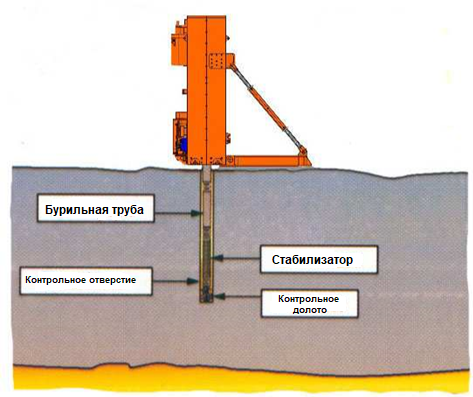
\includegraphics[width=\textwidth]{assets/1121}
		\caption*{Рис. 1- Бурение направляющей скважины станком «RHINO 2007 DC»}
    \end{subfigure}
    \hfill
    \begin{subfigure}[b]{0.45\textwidth}
        \centering
        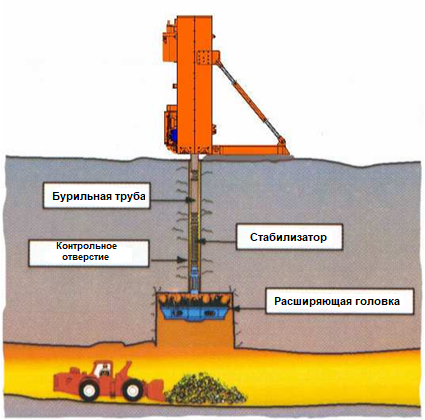
\includegraphics[width=\textwidth]{assets/1122}
		\caption*{Рис. 2 - Разбуривание направляющей скважины до проектного диаметра «RHINO 2007 DC»}
    \end{subfigure}
\end{figure}

\begin{multicols}{2}
Далее с бурильной колонны снимается пилотное долото, затем монтируется
расширительная головка. После скважину бурят до необходимого по проекту
диаметра (рисунок 2).

Нынешний технологии легко позволяют производить бурение восстающих
стволов диаметром 3-4 метра. Однако, что касается бурения более крупных
диаметров, стоит отметить, что внедрение этой технологии идет довольно
медленно. Несмотря на это, использование расширительных головок и
передовых технологий в бурении позволяет достичь более высокой
производительности при бурении стволов диаметром 5-6 метров с
положительным экономическим эффектом, чем это было ранее {[}3{]}.

Результаты многолетних исследований обеспечивают научно-методические
основы для проектирования и расчета жестких и канатных армировок
вертикальных стволов в различных условиях. Были разработаны
безрасстрельные схемы армирования, методы крепления несущих элементов
армировки на анкерах, а также конструкции армировки с ограниченной
податливостью и возможностью радиального регулирования. В тот же период
эти решения были адаптированы для использования в стволах с монолитной
бетонной крепью. Однако теоретические и практические вопросы, связанные
с изучением совместной работы жесткой армировки и набрызгбетонной крепи,
остаются неизученными {[}5{]}.

Набрызгбетонная крепь характеризуется минимальной толщиной,
значительными отклонениями и неровностью контура, что создает сложности
при использовании стандартных жестких армировок ярусного типа и
негативно влияет на её прочностные и деформационные характеристики.
Несущие элементы армировки закрепляются в самой крепи и в окружающем
породном массиве, воздействие которого в существующих методиках расчета
армировки не учитывается. Кроме того, динамические воздействия от
движущихся подъемных сосудов не рассматриваются при определении
параметров набрызгбетонной крепи. Таким образом, возникает необходимость
в комплексном рассмотрении системы "безъярусная армировка -
набрызгбетонная крепь - породный массив" и последующем поиске и
обосновании эффективных решений для армирования глубоких вентиляционных
стволов.

Для крепления вертикальных выработок круглой формы при использовании
обычного метода проходки чаще всего используется монолитный бетон или в
некоторых случаях оставляется без крепления. В устьях и на участках,
проходимых специальными способами в слабых обводненных породах,
устанавливается металлическая тюбинговая крепь. Кроме того, в
зависимости от горно-геологических условий, вертикальные выработки по
всей длине могут быть закреплены железобетонной монолитной, тюбинговой
или набрызгбетонной крепями, а также временной штанговой (анкерной)
крепью с последующим усилением её постоянной бетонной или
набрызгбетонной крепью {[}5{]}.

При выборе конструкции и материала для крепи вертикальных стволов,
инженеры исходят из детального анализа геологических характеристик пород
и условий их расположения, таких как угол падения, трещиноватость и
другие факторы. Результаты исследований основных физико-механических
свойств окружающих пород позволяют определить прочность, угол
внутреннего трения, модуль упругости, пористость и другие характеристики
массива. Эти данные получают на основе изучения геологических
материалов, полученных в результате бурения контрольных разведочных
скважин. Кроме того, ценным и достаточно достоверным источником
информации при выборе конструкции крепи, особенно её толщины, является
обследование и анализ состояния крепи ранее построенных вертикальных
выработок в аналогичных горно-геологических условиях.

Выбор и расчет параметров податливой металлической рамной крепи горных
выработок вне зоны и в зоне влияния очистных работ по пологим,
наклонным, круто-наклонным и крутым платам определяют по Инструкции,
разработанной ВНИМИ в 1991 году.

По методике ВНИМИ, для прогноза устойчивости горизонтальных выработок
угольных шахт в качестве критерия устойчивости принимается величина
ожидаемых смещений на контуре сечения незакрепленной выработки за весь
срок ее службы, определяемых по формуле:

\begin{equation}
u = K_{\alpha} * K_{\theta} * K_{s} * K_{B} * K_{t} * U, \text{мм}_{T}
\end{equation}

где u\textsubscript{т} - смещения (типовые), определяемые по графикам
(рисунок Д.1);

\begin{figure}[H]
	\centering
	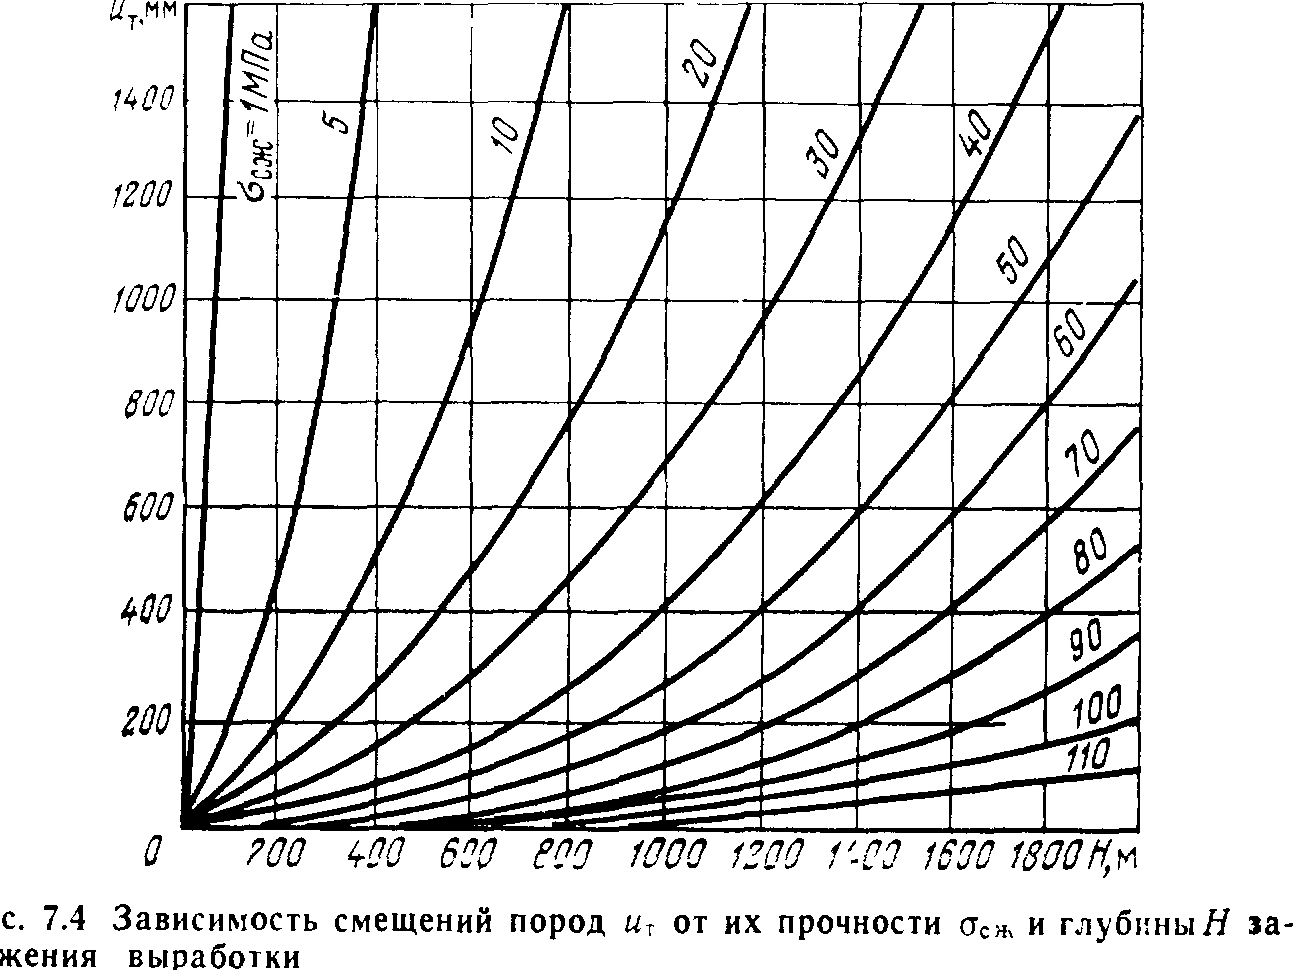
\includegraphics[width=\linewidth]{assets/1124}
	\caption*{Рис. 1 - Графики для определения типовых смещений пород}
\end{figure}

К\textsubscript{α} -коэффициент влияния угла залегания пород и
на­правления проведения выработки относительно простирания по­род или
основных плоскостей трещиноватости, определяемый по таблице 1;

К\textsubscript{θ}-коэффициент, учитывающий направление сме­щений пород и
принимающий значение 1 при определении сме­щений со стороны кровли или
почвы (в вертикальном направ­лении). При определении боковых смещений
пород (в горизон­тальном направлении) К\textsubscript{θ} принимается по
таблице 1.
\end{multicols}

\begin{table}[H]
\caption*{Таблица 1 - Определение боковых смещений пород (в горизонтальном направлении)}
\centering
\begin{tabular}{|p{0.25\textwidth}|lrrrrrrrrr|}
\hline
\multirow{3}{=}{Направление проходки выработки} & \multicolumn{10}{l|}{Коэффициенты К и К в зависимости от угла падения пород, град} \\ \cline{2-11}
 & \multicolumn{2}{l|}{до 20} & \multicolumn{2}{l|}{21-30} & \multicolumn{2}{l|}{31-40} & \multicolumn{2}{l|}{41-50} & \multicolumn{2}{l|}{более 50} \\ \cline{2-11}
 & \multicolumn{1}{l|}{К$_{\alpha}$} & \multicolumn{1}{l|}{К$_{\theta}$} & \multicolumn{1}{l|}{К$_{\alpha}$} & \multicolumn{1}{l|}{К$_{\theta}$} & \multicolumn{1}{l|}{К$_{\alpha}$} & \multicolumn{1}{l|}{К$_{\theta}$} & \multicolumn{1}{l|}{К$_{\alpha}$} & \multicolumn{1}{l|}{К$_{\theta}$} & \multicolumn{1}{l|}{К$_{\alpha}$} & \multicolumn{1}{l|}{К$_{\theta}$} \\ \hline
По простиранию & \multicolumn{1}{r|}{1} & \multicolumn{1}{r|}{0,35} & \multicolumn{1}{r|}{0,95} & \multicolumn{1}{r|}{0,55} & \multicolumn{1}{r|}{0,8} & \multicolumn{1}{r|}{0,8} & \multicolumn{1}{r|}{0,65} & \multicolumn{1}{r|}{1,2} & \multicolumn{1}{r|}{0,6} & 1,5 \\ \hline
вкрест простирания & \multicolumn{1}{r|}{0,7} & \multicolumn{1}{r|}{0,55} & \multicolumn{1}{r|}{0,6} & \multicolumn{1}{r|}{0,8} & \multicolumn{1}{r|}{0,45} & \multicolumn{1}{r|}{0,95} & \multicolumn{1}{r|}{0,25} & \multicolumn{1}{r|}{0,95} & \multicolumn{1}{r|}{0,2} & 0,8 \\ \hline
под углом к простиранию & \multicolumn{1}{r|}{0,85} & \multicolumn{1}{r|}{0,45} & \multicolumn{1}{r|}{0,8} & \multicolumn{1}{r|}{0,65} & \multicolumn{1}{r|}{0,65} & \multicolumn{1}{r|}{0,9} & \multicolumn{1}{r|}{0,45} & \multicolumn{1}{r|}{1,05} & \multicolumn{1}{r|}{0,35} & 1,1 \\ \hline
\end{tabular}
\end{table}

\begin{multicols}{2}
К\textsubscript{S} - ко­эффициент влияния пролета выработки для кровли и
почвы принимается равным К\textsubscript{S} \emph{=} 0,2 (b-1), для
боков выработки К\textsubscript{S} \emph{=} 0,2 (h-1) (b - пролет
выработки, h- высота выработки);

К\textsubscript{В} - коэффициент влияния других вы­работок, равный для
одиночных выработок 1; для сопряжений с односторонним примыканием
выработки-1,4; для сложных сопряжений с примыканием выработок в виде
двустороннего заезда или пересекающихся выработок-1,6. Для параллель­ных
выработок этот коэффициент равен:

\begin{equation}
K_{b} = \frac{(b_1+b_2)*K_L}{L}
\end{equation}

где L- расстояние между выработками, м;

b\textsubscript{1} и b\textsubscript{2} пролеты взаимовлияющих
выработок, м

К\textsubscript{L} коэффициент, принимаемый по табл. 2;

К\textsubscript{t} - коэффициент влияния времени, принимаемый равным 1
для выработок, срок службы которых более 15 лет, и по графикам 2, 3.
\end{multicols}

\begin{figure}[H]
    \centering
    \begin{subfigure}[b]{0.4\textwidth}
        \centering
        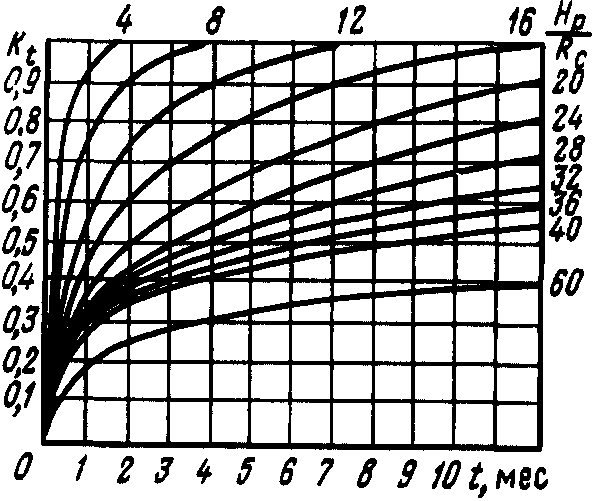
\includegraphics[width=\textwidth]{assets/1126}
		\caption*{Рис. 2 - Графики для определения коэффициента К\textsubscript{t} при сроке службы выработки более года}
    \end{subfigure}
    \hfill
    \begin{subfigure}[b]{0.55\textwidth}
        \centering
        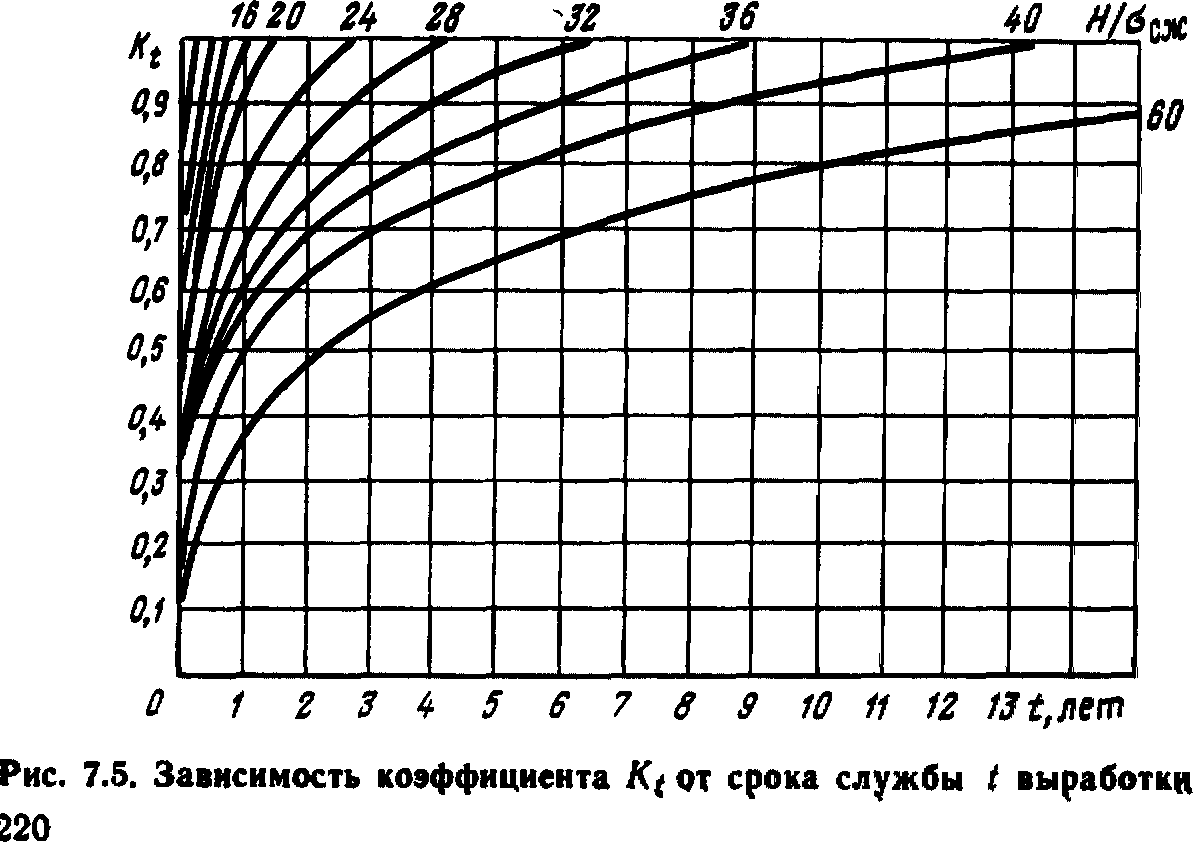
\includegraphics[width=\textwidth]{assets/1127}
		\caption*{Рис. 3 - Графики для определения коэффициента К\textsubscript{t} при сроке службы выработки менее года}
    \end{subfigure}
\end{figure}

\begin{multicols}{2}
Согласно Инструкции ВНИМИ расчетная нагрузка \emph{P} на крепь выработок
как вне зоны влияния очистных работ, так и в зоне влияния очистных работ
определяется исходя из расчетной величины смещений пород кровли, почвы и
боков выработки. Плотность \emph{n} установки рам металлической
податливой крепи на 1 м длины выработки определяют из выражения:

\begin{equation}
n \geq \frac{P}{P_{\text{н}}}
\end{equation}

где \emph{P} -- расчетная нагрузка, к\emph{Н}:

\emph{P}\textsubscript{н} -- несущая способность (сопротивление) рамы,
к\emph{Н}.

Инструкцией предлагается паспортную плотность установки крепи принимать
по ближайшему значению числа рам \emph{n} на 1 м длины выработки в ряду:
0,8; 1; 1,25; 1,33; 1,43; 1,67; 2; 2,25; 2,5; 2,67; 3; 4. Предельной
плотностью податливой металлической рамной крепи рекомендуется считать 3
рамы/м. Методика определения смещений пород в горных выработках,
охраняемых различными способами и испытывающих влияние очистных работ,
изложена в Инструкции.

Нормативные нагрузки на незамкнутую крепь определяют по графикам рис 4 в
зависимости от смещений пород U и ширины выработки в проходке. Если
свойства пород в боках выработки различны, то ожидаемые смещения U и
определяемые по смещениям нормативные нагрузки боковые нагрузки также
будут отличаться друг от друга. В этом случае для дальнейших расчетов
принимают усредненное значение нормативной нагрузки со стороны боков и
нормативную нагрузку со стороны почвы.

Нормативные нагрузки на замкнутую крепь также определяются по графикам
рис. 4 отдельно для кровли, почвы и боков. Усредненная вертикальная
нагрузка определяется по значениям нормативных нагрузок со стороны
кровли и почвы, усредненная горизонтальная нагрузка - по значениям
нормативных нагрузок со стороны боков.
\end{multicols}

\begin{figure}[H]
	\centering
	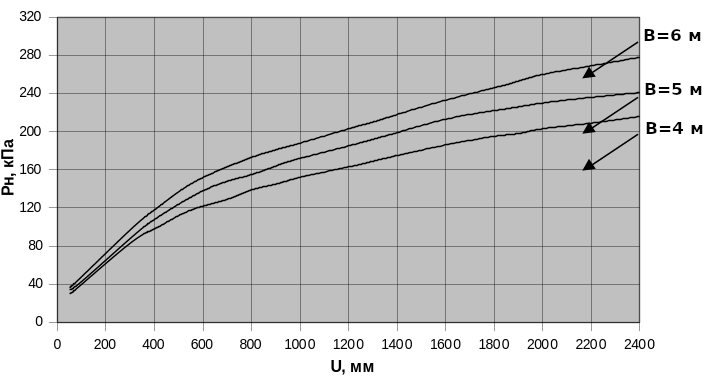
\includegraphics[width=0.8\textwidth]{assets/1360}
	\caption*{Рис. 4 -- Графики определения нормативной нагрузки на крепь}
\end{figure}

\begin{table}[H]
\caption*{Таблица 3 - Значения коэффициента k\textsubscript{п}}
\centering
\begin{tabular}{|l|ll|}
\hline
\multirow{2}{*}{U, мм} & \multicolumn{2}{l|}{значения k\tsb{п} для выработок} \\ \cline{2-3}
 & \multicolumn{1}{l|}{вскрывающих} & Подготавливающих \\ \hline
до 50 & \multicolumn{1}{l|}{1,25} & 1,1 \\ \hline
51-200 & \multicolumn{1}{l|}{1,1} & 1,05 \\ \hline
201-500 & \multicolumn{1}{l|}{1,05} & 1 \\ \hline
более 500 & \multicolumn{1}{l|}{1} & 1 \\ \hline
\end{tabular}
\end{table}

\begin{table}[H]
\caption*{Таблица 4 - Значения коэффициента k\textsubscript{пр}}
\centering
\begin{tabular}{|l|l|l|l|l|}
\hline
\textbf{Н\tsb{р}/R\tsb{c}} & до 16 & более 16 до 20 & более 20 до 25 & более 25 \\ \hline
\textbf{k\tsb{пр}} & 0,6 & 0,8 & 1 & 1,1 \\ \hline
\end{tabular}
\end{table}

\begin{multicols}{2}
Расчетная нагрузка на 1 м выработки со стороны боков определяется по
формуле:

\begin{equation}
P_{\text{в}}=k_{\text{п}}  * k_{\text{н}}  * k_{\text{пр}}  * Р_{\text{в}}^{\text{н}}, \text{кПа}
\end{equation}

где k\textsubscript{п}- коэффициент перегрузки, учитывающий изменчивость
нагрузки (таблица 3);

k\textsubscript{н}- коэффициент, принимаемый для главных вскрывающих
выработок равным 1,1; для остальных-1;

k\textsubscript{пр}- коэффициент условий проведения выработок,
принимаемый равным 1 при проведении выработок буровзрывным способом. При
комбай­новом способе проведения выработок принимается по таблице 4;

Р\textsuperscript{н}\textsubscript{в}- нормативная вертикальная
нагрузка.

Если свойства пород в боках выработки различны, то ожидаемые смещения U
и определяемые по смещениям нормативные нагрузки боковые нагрузки также
будут отличаться друг от друга.

Расчетная нагрузка на 1 м выработки со стороны боков определяется по
формуле:

\begin{equation}
P_{\text{в}}=k_{\text{б}}  * k_{\text{н}}  * k_{\text{пр}}  * Р_{\text{б}}^{\text{н}}, \text{кПа}
\end{equation}

где Р\textsuperscript{н}\textsubscript{б}- нормативная горизонтальная
нагрузка, кПа.

{\bfseries Результаты и обсуждение.} Технический результат заключается в
повышении эффективности крепления шахтного ствола за счет конструкции,
включающей в себя кольцевую крепь, размещённую в специальной нише
ствола, закрепленную анкерами. Для предотвращения вывалов породы,
устанавливается сетка, в местах геологических нарушений дополнительно
применяется набрызгбетонная крепь {[}6{]}.

В пройденном участке устья ствола монтируется подвесной проходческий
полок, для чего предусматривается установить временное перекрытие для
монтажа проходческого полка.

Крепление участка устья ствола производится монолитным железобетоном с
помощью инвентарной опалубки с рабочей высотой 0,9÷1,0 м

Постоянная крепь пройденного ранее участка устья ствола возводится после
сооружения опорного венца снизу-вверх. Бетон подается за опалубку по
временным ставам бетонопроводов, подвешенными на лебедках забойного
бетонопровода. Для равномерной укладки бетона по всему периметру ствола
на концы бетонопроводов навешиваются гибкие гофрированные рукава
необходимого диаметра.

По мере возведения постоянной крепи временную крепь демонтируют и
извлекают на поверхность. \emph{{\bfseries Бетонированию}} подлежат боковые
породы за контуром постоянной железобетонной крепи на устье ствола
{[}7{]}.

Кольцевая крепь представляет собой разновидность рамной крепи с
замкнутым контуром, состоящей из отдельных колец, установленных вдоль
выработки вразбежку и связанных между собой при помощи стяжек (подвесок)
или распорок, и применяемой в горизонтальных, наклонных и вертикальных
выработках при наличии всестороннего смещения массива горных пород.
Кольцевую крепь классифицируют по площади сечения выработок (от 6,5 до
20,1 м), по конструктивному исполнению (жесткие, шарнирные и податливые)
и применяемому прокату и марке стали {[}8{]}.
\end{multicols}

\begin{figure}[H]
    \centering
    \begin{subfigure}[b]{0.45\textwidth}
        \centering
        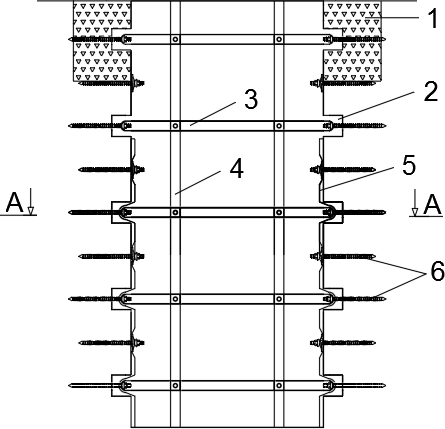
\includegraphics[width=0.75\textwidth]{assets/1131}
    \end{subfigure}
    \hfill
    \begin{subfigure}[b]{0.4\textwidth}
        \centering
        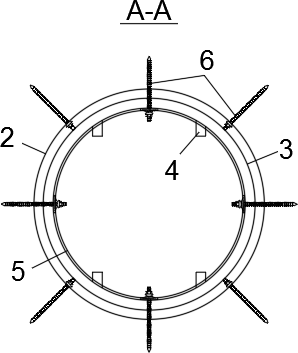
\includegraphics[width=0.75\textwidth]{assets/1132}
    \end{subfigure}
    \caption*{Рис. 3 - Разработанная технология крепления ствола}
\end{figure}

\begin{multicols}{2}
Устье ствола 1 бетонируется. В месте монтажа кольцевой крепи выбирается
ниша 2 диаметром не менее R+300 мм, где R -- диаметр ствола. В нишу
устанавливается кольцевая крепь 3. Кольцевая крепь между собой соединена
при помощи стальных расстрелов и проводников 4 {[}9{]}.

Далее устанавливается пластиковая либо металлическая сетка 5 (для
предотвращение осыпаний), после чего производится крепление анкерами 6,
как кольцевой крепи, так и межрамного пространства (Рисунок 3).

Процесс установки анкеров включает несколько этапов, таких как бурение
шпуров, подготовка раствора, наполнение шпуров раствором и закладка
арматурных стержней. Расположение шпуров для установки штанг должно
соответствовать указаниям в паспорте крепления.

При установке анкеров через металлическую сетку, которую необходимо
закрепить в углублениях породного обнажения, допускается отклонение
расстояния между анкерами до 30 \%.

Для обеспечения надежного сцепления цементно-песчаного раствора с
породой в стенках шпуров, необходимо тщательно продуть шпуры сжатым
воздухом или промыть их водой с целью полного удаления буровой мелочи и
пыли.

Цементно-песчаный раствор для анкеров готовят с использованием
растворомешалки или вручную, после чего подают в шпур при помощи
пневмонагнетателя сжатым воздухом через резиновый шланг и металлическую
трубу диаметром 18-25 мм. Длина трубы должна быть не меньше глубины
шпура. Трубку вводят в шпур до его забоя, и в процессе заполнения шпура
раствором её постепенно вытаскивают из шпура {[}10{]}.

Процедура заполнения шпура раствором должна обеспечивать полное
закрепление анкера по всей его длине.

{\bfseries Выводы.} Проведенный анализ технических и технологических
решений крепи и армировки стволов позволил сформулировать объект и
предмет, область применения научных и практических результатов, а также
сделать следующие основные выводы:

1. В вентиляционных стволах угольных шахт и рудников, отнесенных к I и
II категории устойчивости, целесообразно применять ресурсосберегающую
набрызгбетонную крепь. Она достаточно широко использовалась в нашей
стране в 70-80 годы прошлого века. Однако в последние 20 лет для
крепления стволов глубиной более 700 м в устойчивых породах применяется
только монолитная бетонная крепь. Одной из причин такого положения
является отсутствие эффективных технических и технологических решений
жесткой армировки, адаптированных для применения в стволах, закрепленных
набрызгбетоном.

2. Канатная армировка может успешно применяться в стволах с любым типом
крепи, но с увеличением их глубины зачастую возникает необходимость
увеличения диаметра ствола, также существенно возрастает масса
направляющих канатов и натяжных устройств, что делает неэффективным ее
применение.

3. Определена область применения кольцевой крепи с упрочняющей анкерной
крепью в более склонных к ползучести аргиллитах. Для ее увеличения
целесообразно применение цементных анкеров с ограниченной податливостью.
\end{multicols}

\begin{center}
{\bfseries Литература}
\end{center}

\begin{noparindent}
1. Геотехнология строительная: методические указания. -Донецк: Донецкий
национальный технический университет, 2017.

2.Технологический регламент (инструкция) по выбору типов и параметров
крепей и технологии их возведения на Артемьевском месторождении --
Караганда: ТОО «Mining Research Group», 2015.-108 с.

3.Бабец, Д.В. Применение метода группового учета аргументов к задаче
оценки устойчивости горной выработки // Горный
информационно-аналитический бюллетень. -2001. - №11. -С. 67-69.

4.Басакевич, С.В. Обоснование параметров безрасстрельной армировки
вертикальных стволов на основе вероятностной оценки временных нагрузок:
дис. ... канд. техн. наук: 25.00.22 / Басакевич Сергей Владимирович. -
Новочеркасск, 2009. - 145 с.

5. Dahlin, T. The development of DC resistivity imaging techniques //
Computers \& Geosciences. -- 2001. - Vol. 27. --P. 1019--1029. DOI
10.1016/S0098-3004(00)00160-6

6. Бобачев, А.А. Электроразведка: пособие по электроразведочной практике
для студентов геофизических специальностей. Том II Малоглубинная
электроразведка. Изд. 2-е, перераб. и доп. / Бобачев А.А. и др. - М.:
МГУ-2013. -123 с. ISBN:~978-5-904807-21-4

7. Груздев А.А., Науменко Д.А.,. Богданов П.С, Бобачев А.А., Шевнин В.А.
Бесконтактное измерение электрического поля с помощью OHMMAPPER в
условиях крайнего севера.// Электронный журнал "Георазрез", -2013. - №
01 (13). -С.1--23.

8. Loke M.H. Tutorial: 2-D and 3-D electrical imaging surveys.- URL :
www.geotomosoft.com (Revision date : 27th August 2021)

9. Адушкин В.В.,Спивак А.А., Кожухов С.А., Кукушкин Ю.В. Резонансные
особенности эсхаляции природного радона// Доклады РАН. -- 2005. - Т.400
(3). - С.369-371.
\end{noparindent}

\begin{center}
{\bfseries References}
\end{center}

\begin{noparindent}
1. Geotekhnologiya stroitel\textquotesingle naya: metodicheskie
ukazaniya. -Donetsk: Donetskii natsional\textquotesingle nyi
tekhnicheskii

universitet, 2017. {[}in Russian{]}

2.Tekhnologicheskii reglament (instruktsiya) po vyboru tipov i
parametrov krepei i tekhnologii ikh vozvedeniya na
Artem\textquotesingle evskom mestorozhdenii -- Karaganda: TOO «Mining
Research Group», 2015.-108 s. {[}in Russian{]}

3.Babets, D.V. Primenenie metoda gruppovogo ucheta argumentov k zadache
otsenki ustoichivosti gornoi vyrabotki // Gornyi
informatsionno-analiticheskii byulleten\textquotesingle. -2001. - №11.
-S. 67-69. {[}in Russian{]}

4.Basakevich, S.V. Obosnovanie parametrov
bezrasstrel\textquotesingle noi armirovki vertikal\textquotesingle nykh
stvolov na osnove veroyatnostnoi otsenki vremennykh nagruzok: dis. ...
kand. tekhn. nauk: 25.00.22 / Basakevich Sergei Vladimirovich. -
Novocherkassk, 2009. - 145 s. {[}in Russian{]}

5. Dahlin, T. The development of DC resistivity imaging techniques //
Computers \& Geosciences. -- 2001. - Vol. 27. --P. 1019--1029. DOI
10.1016/S0098-3004(00)00160-6 {[}in Russian{]}c

6. Bobachev, A.A. Elektrorazvedka: posobie po elektrorazvedochnoi
praktike dlya studentov geofizicheskikh spetsial\textquotesingle nostei.
Tom II Maloglubinnaya elektrorazvedka. Izd. 2-e, pererab. i dop. /
Bobachev A.A. i dr. - M.: MGU-2013. -123 s. ISBN: 978-5-904807-21-4
{[}in Russian{]}

7. Gruzdev A.A., Naumenko D.A.,. Bogdanov P.S, Bobachev A.A., Shevnin
V.A. Beskontaktnoe izmerenie elektricheskogo polya s
pomoshch\textquotesingle yu OHMMAPPER v usloviyakh krainego severa.//
Elektronnyi zhurnal "Georazrez", -2013. - № 01 (13). -S.1--23. {[}in
Russian{]}

8. Loke M.H. Tutorial: 2-D and 3-D electrical imaging surveys.- URL :
www.geotomosoft.com (Revision date : 27th August 2021)

9. Adushkin V.V.,Spivak A.A., Kozhukhov S.A., Kukushkin Yu.V.
Rezonansnye osobennosti eskhalyatsii prirodnogo radona// Doklady RAN. --
2005. - T.400 (3). - S.369-371. {[}in Russian{]}
\end{noparindent}

\emph{{\bfseries Сведения об авторах}}

\begin{noparindent}
Мусин Р. А. -PhD доктор, и.о. доцента, Карагандинский технический
университет имени Абылкаса Сагинова, Караганда, Казахстан, e-mail:
R.A.Mussin@mail.ru;

Асанова Ж.М. - PhD доктор, и.о. доцента, Карагандинский технический
университет имени Абылкаса Сагинова, Караганда, Казахстан, e-mail:
zhanar-a@bk.ru;

Байкенжин М. А. - PhD доктор, доцент, Карагандинский технический
университет имени Абылкаса Сагинова, Караганда, Казахстан, e-mail:
nailzamaliev@mail.ru

Альжанов Р.Х. - докторант группы ГДД-21, Карагандинский технический
университет имени Абылкаса Сагинова, Караганда, Казахстан, e-mail:
rushair@mail.ru.
\end{noparindent}

\emph{{\bfseries Information about the authors}}

\begin{noparindent}
Musin R. A. - PhD, acting Associate Professor of the Abylkas Saginov
Karaganda Technical University, Karaganda, Kazakhstan, e-mail:
R.A.Mussin@mail.ru;

Asanova Zh. M.- PhD, acting Associate Professor of the Abylkas Saginov
Karaganda Technical University, Karaganda, Kazakhstan, e-mail:
zhanar-a@bk.ru;

Baikenzhin M. A.- candidate of technical sciences, associate professor
of the Abylkas Saginov Karaganda Technical University, Karaganda,
Kazakhstan, e-mail: mbmqm@mail.ru;

Alzhanov R.H. - doctoral student group GDD-21 Abylkas Saginov Karaganda
Technical University, Karaganda, Kazakhstan, e-mail: rushair@mail.ru.
\end{noparindent}
